\chapter{Cloud Computing}
\label{cha:fundamentacao_teorica}

Muitas são as definições encontradas nos trabalhos atuais para cloud computing
\cite{article-learning-as-a-service}, porém será adotada para este trabalho a mesma definição utilizada
por este autor, que foi criada pelo \emph{NIST} (Instituto Nacional de Padrões e Tecnologia dos Estados
Unidos da América). Em \citeonline{nist-cloud-computing}, o NIST define \emph{cloud computing} como:
``um modelo acesso via rede, ubíquo, conveniente e sob-demanda a uma pilha de recursos computacionais
configuráveis (redes, servidores, armazenamento e serviços) que podem ser rapidamente provisionados e
lançados com o mínimo de esforço em gerenciamento ou interação com o provedor de serviços''. Também
são definidos pelo NIST quatro modelos de implantação de \emph{cloud computing}:

\begin{description}
    \item[Private cloud (nuvem privada)] é provisionada e utilizada por uma única
    organização. Pode pertencer e ser gerenciada pela própria organização, terceiros,
    ou uma combinação destes e estar dentro ou fora dos limites físicos da
    organização.

    \item[Community cloud (nuvem comunitária)] é provisionada e utilizada por uma
    comunidade de organizações que tem interesses comuns. Pode pertencer e ser gerneciada
    por uma das organizações, terceiros ou uma combinação destes e estar dentro ou fora
    dos limites físicos da organização.

    \item[Public cloud (nuvem pública)] é privisionada para o uso do público em geral.
    Pode pertencer e ser gerenciada por uma empresa, instituição de ensino ou governamental,
    ou uma combinação destes e estar dentro dos limites físicos do seu provedor.

    \item[Hybrid cloud (nuvem híbrida)] uma composição de dois ou mais dos modelos
    já mencionados que mantêm-se entidades únicas, porém são ligadas por tecnologia
    padronizada ou proprietária que possibilita compartilhamento de recursos entre
    elas.
\end{description}

Algumas características são essenciais ao cloud computing, segundo
\citeonline{article-learning-as-a-service}: \textit{self-service} sob-demanda, um
consumidor do serviço pode provisionar seus recursos sem a necessidade de intervenção
humana; acesso a rede de banda larga, que será o meio por onde o cliente se comunicará e
acessará o serviço requisitado através de mecanismos padronizados, que permitam que isto
seja feito a partir de smartphones, notebooks, etc; \textit{pool} de recursos, onde os recursos
físicos são frequentemente utilizados através de um \textit{pooling} para servir a múltiplos clientes
com diferentes recursos físicos e virtuais dinamicamente determinados pelos próprios clientes;
rapida elasticidade, onde estes recursos virtuais podem ter suas capacidades rapidamente
modificadas e provisionadas, até mesmo automaticamente, tanto para cima quanto para baixo;
e serviço mensurado, onde o provedor pode controlar e otimizar o uso de recursos físicos
através de um sistema de mensuração em algum nível do ambiente.

Este mesmo autor ainda diz que o cloud computing só se tornou realizável graças a
outras 4 tecnologias já existentes:

\begin{description}
    \item[Virtualização] possibilita a criação de recursos computacionais virtualizados
    (redes, servidores e/ou armazenamento). Oferece consolidação dos recursos computacionais
    físicos, separação e proteção.

    \item[Grid computing] possiblita a execução de tarefas em múltiplos computadores
    dispersos, fornecendo de maneira transparente a capacidade de um supercomputador.

    \item[Utility computing] possibilita o empacotamento e provisionamento dos recursos
    computacionais virtualizados através de um serviço de mensuração e um sistema de
    preços para que estes sejam oferecidos sob-demanda.

    \item[Web Service] são ``pedaços'' de \emph{software} que são publicados e num registro
    para serem descobertos dinamicamente e usados por outros \emph{softwares} através de um
    protocolo de transporte (HTTP, TCP/IP, etc) independente da plataforma ou linguagem
    de programação.
\end{description}

Dentro do conceito de \emph{cloud computing}, o NIST identificou 3 tipos de serviços básicos que este
modelo de computação é capaz de oferecer. São eles:

\begin{itemize}
    \item Infraestrutura como serviço (IaaS): são oferecidos recursos computacionais de base,
    como redes, servidores e armazenamento através da rede. Possibilitando todos o poder
    de gerenciamento de um servidor físico, porém livrando seu usuário das preocupações
    relacionadas ao \emph{hardware} do servidor.

    \item Plataforma como serviço (PaaS): oferece ambientes pré-configurados com determinados
    softwares, para que os desenvolvedores possam facilmente desenvolver suas soluções
    usando-os e publicá-las sem as complicações de ter que gerenciar manualmente um servidor
    com todos estes softwares.

    \item Software como serviço (SaaS): esta camada oferece um software usável diretamente
    ao cliente, com total transparência do servidor ou plataforma necessário para este. Tudo é devidamente
    abstraído e gerenciado pelas ferramentas usadas no cloud computing. Os softwares oferecidos
    podem ser os mais diversos, como aplicações de produtividade ou Gestão de Relacionamento
    com o Cliente (CRM).

\end{itemize}

Cada um destes modelos é usado como base para o modelo acima poder oferecer um serviço
que terá mais valor para o cliente leigo, vide Figura \ref{img:piramide-cloud}. Assim,
entende-se que quando um desenvolvedor faz uso do seu serviço de PaaS, podem ser instanciadas
várias unidades de IaaS e quando um cliente faz uso do SaaS, várias instâncias de PaaS (e,
consequentemente, IaaS) podem ser criadas. A quantidade de instâncias de nível inferior
necessárias depende das configurações determinadas para cada item dentro do serviço
requisitado.

\begin{figure}[h]
  \center
  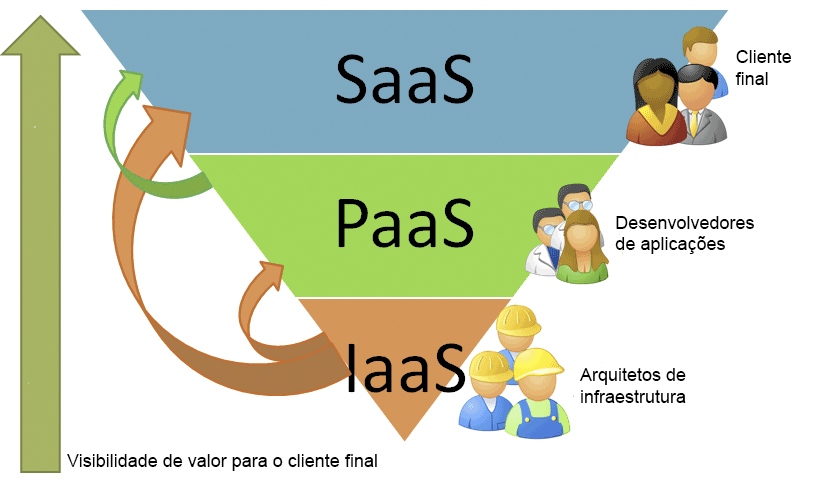
\includegraphics[scale=0.35]{imagem/piramide-cloud.png}
  \caption{Pirâmide representando os 3 serviços oferecidos por uma cloud}
  \label{img:piramide-cloud}
\end{figure}

\section{Virtualização}

Virtualização é a técnica que permite particionar um único sistema computacional em
vários outros, denominados máquinas virtuais \cite{virt-teoria-solucoes}. Segundo
este mesmo autor, estas máquinas virtuais oferecem um ambiente extremamente similar ao de uma máquina física.
Possuem seu próprio sistema operacional, aplicativos e serviços de rede. Ainda é possível
conectar um conjunto dessas máquinas virtuais através redes, switches ou roteadores virtualizados.

São diversas as tecnologias que implementam a virtualização de recursos computacionais.
Alguns dos mais conhecidos e evoluídos softwares desta área são: Hyper-V, Xen, KVM,
VMWare ESXi. \citeonline{virt-con-aplica} definem 3 partes básicas que podem ser
observadas em um ambiente de virtualização:

\begin{enumerate}
    \item
        O sistema nativo (real), conhecido também como sistema hospedeiro, que contém todo o hardware
        físico;

    \item
        O sistema virtual, conhecido também como sistema convidado, que executa o sistema virtualizado,
        simulando a maioria dos recursos de hardware que um sistema nativo poderia ter;

    \item
        A camada de virtualização, conhecida como \textit{hipervisor}, que faz a comunicação entre a
        interface virtual e nativa. Esta camada é representada pelos softwares de virtualização, como
        os já mencionados Hyper-V, Xen, KVM e VMWare ESXi.
\end{enumerate}

Este mesmo autor ainda diz que \emph{hipervisors} são mais complexos do que podem
parecer, por exemplo, caso o conjunto de instruções da máquina virtual e da real
sejam diferente (Linux virtualizado dentro de um Windows, ou vice-versa) haverá
a necessidade da conversão de instruções pela CPU da máquina real. É necessário
também mapear os recursos de hardware da máquina real (como mouses,
armazenamento externo, etc) que poderão ser acessados pela máquina virtual. Contudo,
todos os \emph{hipervisors} conhecidos já são extremamente evoluídos e lidam
muito bem com todas as complicações necessárias para possibilitar uma virtualização
adequada.

\citeonline{virt-teoria-solucoes} diz que é comum encontrarmos infra-estruturas com a filosofia de "um servidor
por serviço", por motivos de heterogeneidade das necessidades dos clientes e, alguns casos, até segurança. Normalmente, este
contexto acaba deixando o processador e alguns outros recursos subutilizados.

A virtualização resolve este problema de subutilização de recursos computacionais,
através do tratamento de ambas suas duas mais comuns causas: a filosofia ``um servidor por serviço'' e
a heterogeniedade das necessidades dos clientes.
Obtém-se diversos sistemas operacionais contidos em apenas um
hardware físico. Com uma máquina virtual disponibilizada para cada serviço, ela pode ter o sistema operacional,
bibliotecas e exatamente a configuração de memória, processador e armazenamento necessários para aquele serviço
funcionar, onde todos estes recursos podem ser inclusive alterados e dimensionados de acordo com o
crescimento ou decrescimento do consumo destes pelo serviço. Resumidamente, temos a flexibilidade, portabilidade,
um melhor aproveitamento dos recursos do hardware físico através do uso da quantidade adequada de máquinas virtuais e
elasticidade de executar diversos serviços diferentes, em sistemas operacionais diferentes, com necessidades de recursos
diferentes e que mudam conforme o tempo dentro, tudo dentro de um mesmo hardware. Este ato é conhecido como consolidação de servidores
e é imensamente importante para \textit{data-centers}, por exemplo, devido a diversas demandas de sistemas operacionais
por seus clientes, menor ocupação de espaço por máquinas físicas, melhor aproveitamento de energia elétrica, refrigeração, cabeamento, etc.

\section{Grid Computing}
\label{sec:grid}

Segundo \citeonline{foster1999grid}, o principal objetivo do
\textit{grid computing} é multiplexar recursos computacionais, de diversos provedores (hardware físico), de maneira
transparente para vários usuários. Desta maneira, o usuário percebe um único super-recurso, que na verdade é composto
por vários outros recursos menores.
\citeonline{grid-virtual-machines}, enunciam que, sistemas tradicionais de computação, por sua vez, multiplexam os
recursos de um único computador para vários usuários através da implementação de contas de usuários pelo
sistema operacional. Este modelo assume que existe uma entidade administrativa 100\%
confiável que possui permissão para adicionar usuários e restringir seu acesso conforme necessário. Enquanto isso,
sistemas de \emph{grid computing} devem possuir vários domínios diferentes, cada qual sua própria entidade administrativa, e não
podem depender de uma autoridade central.

\citeonline{grid-cloud-compared} nos mostram que a definição de \emph{cloud computing}
sobrepõe a de muitas tecnologias recentes, incluindo \emph{grid computing},
\emph{utility computing} e até \textit{web services} (estes dois últimos serão
devidamente mencionados nas duas próximas subseções). Segundo ele,
a definição de \emph{cloud computing} não só sobrepõe a de \emph{grid computing}, ela é de fato uma forma evoluída do
\emph{grid computing} e usa-o como base para seu funcionamento. Tal evolução teve como motivação a mudança do foco, que
antes era de infraestrutura para armazenamento e recursos de processamento, para recursos mais abstratos e serviços que apresentam um maior valor para seus usuários.

A sobreposição dos conceitos e a mudança de foco podem ser melhor entendidos visualizando a Figura \ref{img:grid-cloud-compared}.
Através dela, é evidente perceber que \emph{grid computing} é um conceito mais focado em aplicações e \emph{cloud computing} em serviços.
Pode-se notar também que \emph{clouds} utilizam \emph{grids} e que \emph{grids}, por sua vez, são baseadas \emph{clusters} de
computadores ou supercomputadores.

\begin{figure}[h]
  \center
  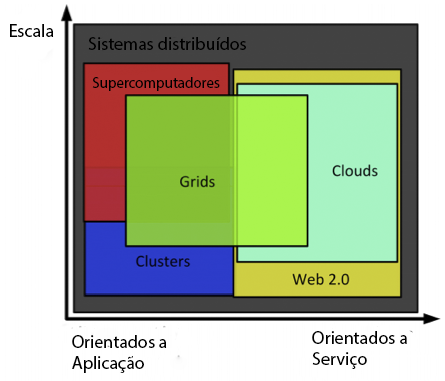
\includegraphics[scale=0.6]{imagem/grid-cloud-compared.png}
  \caption{Comparação de \emph{grid} e \emph{cloud computing}, mostrando a sobreposição dos conceitos}
  \caption*{Fonte: \citeonline{grid-cloud-compared}}
  \label{img:grid-cloud-compared}
\end{figure}

De acordo com \citeonline{grid-checklist}, a essência das definições do \emph{grid computing} pode ser capturada de
maneira simples em 3 itens:

\begin{enumerate}
    \item
        É composta por recursos coordenados que não dependem de um controle centralizado. Ela integra e
        coordena recursos e usuário de diferentes domínios de controle, por exemplo, diferentes unidades
        administrativas da mesma compania, ou até mesmo diferentes companias, cuidando de tudo que  diz
        respeito a segurança, políticas de acesso e qualquer outra configuração que venha a surgir de acordo
        com o contexto;

    \item
        Usa protocolos e interfaces padronizados, abertos e de propósito geral. Todos estes itens
        devem tratar problemas fundamentais, como autenticação, autorização, descoberta e acesso a
        recursos. É muito importante que estes protocolos e interfaces sejam abertos, caso contrário
        o sistema seria específico para determinada aplicação;

    \item
        Oferece uma qualidade de serviço não-trivial. Uma \emph{grid} permite que seus recursos sejam
        coordenados de maneira a entregar qualidades de serviço complexas, relacionadas a
        tempos de resposta, \textit{throughput}, avaliabilidade, segurança e co-alocação
        de múltiplos recursos para satisfazer as demandas de seus usuários. Assim, o sistema
        como um combinado tem uma utilidade maior que a soma de suas partes.

\end{enumerate}

\section{Utility Computing}

Segundo \citeonline{utility-market}, as técnicas tradicionais de gerenciamento de recursos
(alocação, controle de admissão e agendamento) se mostraram inadequadas para \emph{grids} compartilhadas,
definidas na Seção \ref{sec:grid}. Estas técnicas de gerenciamento de recursos não
fornecem facilidades para usuários requisitarem os recursos demandados de maneira apropriada e não refletem o valor,
importância e prazos da necessidade do usuário. Este problema ainda afeta diretamente os provedores
de \emph{grids} compartilhadas, já que não oferece nenhuma forma de seus contratantes serem compensados pelos recursos
compartilhados com outras entidades.

Não há como garantir que determinados usuários tenham acesso dedicado e com certos
níveis de qualidade de serviço e uma determinada gama de recursos, como processamento, memória e
armazenamento, não conseguindo extrapolar este limite. Pesquisadores e entusiastas encontraram
técnicas de gerenciamento de recursos baseadas no mercado que resolvem essas limitações. Tais
técnicas tem como objetivo fornecer um \emph{framework} para incentivar
os provedores de serviços priorizar a tarefas de maior importância, urgência e utilidade.
Este \emph{framework}, por sua vez, atua como \textit{middleware} em sistemas de \emph{grid computing}
garantindo que todos os conceitos de \emph{utility computing} sejam aplicados e respeitados
dentro daquele ambiente.

\begin{citacao}
    Existem muitas abordagens com relação ao \emph{utility computing}. Amplamente, elas se dividem
    em duas categorias. A primeira é o modelo de \textit{utilidade compartilhada}, onde
    os recursos são utilizados por diversos clientes ao mesmo tempo. A segunda, mais recente,
    é definida como modelo de \textit{utilidade de servidor completo}, onde aplicações
    programaticamente adquirirem e liberam o servidor conforme for necessário.
    \cite{utility-computing-models}
\end{citacao}

Para melhor entender as diferenças entre os modelos de utilidade compartilhada e
de servidor completo, temos a Figura \ref{img:utilidade-compartilhada}, demonstrando
um modelo de utilidade compartilhada. Nele, cargas de trabalho são entregues
a uma central de processamento, que irá distribuí-las entre vários servidores
(unidades de processamento compartilhado). Já para exemplificar o modelo de servidor
completo, temo a Figura \ref{img:utilidade-servidor-completo}: neste modelo,
aplicações são delegadas a um ou mais servidores exclusivos (de acordo com a
carga de processamento que esta aplicação necessita no momento), que processam nada
além destas aplicações a eles atribuídas.

\begin{figure}[h]
  \center
  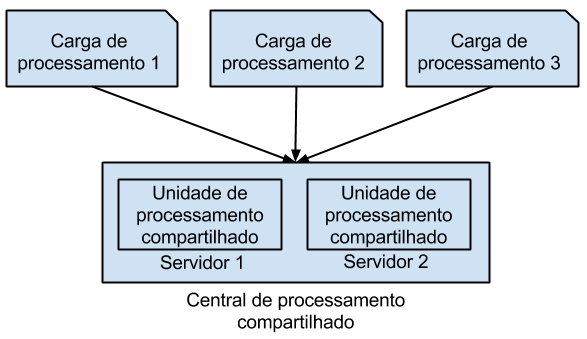
\includegraphics[scale=0.7]{imagem/utilidade-compartilhada.png}
  \caption{Modelo de utilidade compartilhada}
  \label{img:utilidade-compartilhada}
\end{figure}

\begin{figure}[h]
  \center
  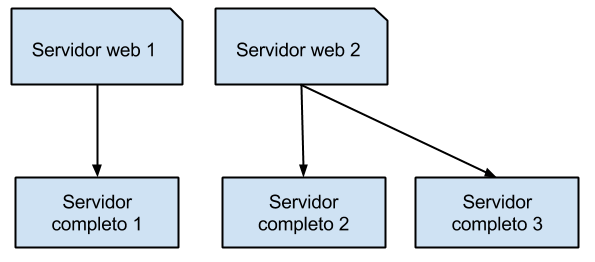
\includegraphics[scale=0.7]{imagem/utilidade-servidor-completo.png}
  \caption{Modelo de utilidade de servidor completo}
  \label{img:utilidade-servidor-completo}
\end{figure}

\section{Web Service}

\citeonline{web-services-distributed} definem
web services como: uma entidade programática que fornece uma funcionalidade particular, como
lógica de aplicação, e é disponibilizado para diversos potenciais usuários através da internet.
Segundo o mesmo, um grande conceito por trás dos \emph{web services} é o de arquiteturas orientadas
a serviços (\textit{service-oriented architecture}, em inglês, ou \emph{SOA}).
\textit{Web services} adicionaram um novo nível de funcionalidade para a atual \textit{Web},
tomando o primeiro passo em direção à integração de componentes de \emph{software} distribuídos
usando padrões da \emph{web} (protocolo HTTP, XML ou JSON, URIs, SOAP, WSDL, etc), definidos pela
\emph{World Wide Web Consortium} (W3C) \cite{book-web-services}.
Tal arquitetura sugere algumas atividades essenciais para o funcionamento dos determinados serviços, assim
como sua utilização por clientes (internos ou externos à organização desenvolvedora do serviço). São elas:

\begin{enumerate}
    \item
        Um serviço deve ser criado, com suas interfaces e métodos de chamada definidos;

    \item
        Ele deve ser publicado, seja em intranet ou internet, para que possíveis
        usuários possam localizá-lo;

    \item
        Deve ser localizável para que possa ser utilizado pelos potenciais usuários;

    \item
        O serviço precisa ser utilizado para que ofereça algum tipo de benefício;

    \item
        E o serviço preciso ser ``despublicado'', quando não é mais necessário ou não
        está mais disponível.
\end{enumerate}

Pode-se ver na Figura \ref{img:fluxo-webservice}, os passos necessários para que um
cliente possa finalmente utilizar um web service. Primeiramente, após construído, este
serviço (\textit{service provider}) deve ser publicado em um índice (chamado de \textit{service broker}).
Então, um cliente (\textit{service requester}), pode acessar o índice e procurar por um serviço
disponível para ele. Após este cliente acessar os dados do índice, ele se conecta diretamente com o
serviço e realiza a comunicação necessária para prosseguir com o uso deste.

\begin{figure}[h]
  \center
  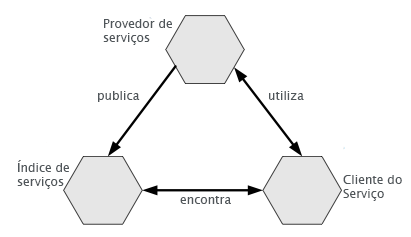
\includegraphics[scale=0.7]{imagem/fluxo-webservice.png}
  \caption{Fluxograma mostrando os passos para publicação, localização e uso de um web service}
  \caption*{Adaptado para português de \citeonline{web-services-distributed}}
  \label{img:fluxo-webservice}
\end{figure}

A comunicação baseada em tecnologias \emph{web} garante a interoperabilidade dos \emph{web
services}, independentemente plataforma em que é desenvolvido ou consultado.
Isto acaba ajudando equipes a desenvolver um software altamente escalável,
programando as partes mais custosas como serviços externos, usando as ferramentas
mais adequadas para que haja o esperado ganho em escalabilidade, ou em legibilidade do código.
Em um ambiente de \emph{cloud computing}, escalabilidade e interoperabilidade são
de suma importância para um aproveitamento eficiente dos recursos computacionais
disponíveis para esta finalidade e garantir o crescimento da \emph{cloud} sem problemas.
É evidente que manter uma parte de um \emph{software} isolada torna a manutenção e evolução
do seu código muito mais simples do que fazer o mesmo no \emph{software} completo, por inteiro.
Cada parte pode ser testada e finamente polida, ainda aproveitando das melhores
ferramentas que determinadas linguagens podem oferecer para a resolução de problemas
específicos.
